\documentclass[
  utf8,%     More capable input encoding than latin-1.
  parskip,%  For vertical whitespace between paragraphs.  This comes down to more than just using parskip.sty, so it's better to use this class option.
  % S5MP % If you intend to really use margin paragraphs (not recommended!).
%  crop,%     Produce output with crop marks and paper size A4.  Liu-Tryck should like this.  Automatically adds information, including the physical page number, at the top of each page.
       %     Add option 'noInfo' to suppress the info at the top of each page when using option 'crop'.
  % Font options: 'kp' (default), 'times', 'lm'.  The KpFonts (loaded using 'kp'), is the most complete font among the provided options.  Among other, it supports slanted small caps.  See rtthesis.cls for more details regarding the font options.
  largesmallcaps,intlimits,widermath,% Good options to KpFonts.
  sharecounter,nobreak,definition=marks,%  See comments in the results chapter of this document for more information on these options!
  %numbers, % If you want to cite references by numbers, use this option.
  noparts % Use option 'noparts' if you do not make use of part divisions.
]{rtthesis}

\usepackage{mythesis}
\usepackage{longtable}

\begin{document}
\selectlanguage{english}
\makeFrontPage
\frontmatter
\title{Genomgång av nya och alternativa krypterings- och scramblingssystem för 
digital-teve samt implementering av ny scrambling-algoritm (AES128) på FPGA}
\author{Gustaf Bengtz}
\maketitle
\makeLibraryPage{This report adresses why the currently used scrambling standard CSA 
needs a replacement. Proposed replacements to CSA are analyzed to some 
extent, and an alternative replacement (AES128) is analyzed.

One alternative being the CSA3, and the other being the CISSA algorithm.
Both of them are based on the public AES algorithm. Both of the 
proposed algorithms use the AES algorithm as a base. The CSA3 combines 
it with a secret cipher, the XRC, while CISSA uses the AES cipher in a 
feedback mode. The different utilizations makes CSA3 hardware friendly 
and CISSA software friendly.

The implementation of the Advanced Encryption Standard (AES) is 
analyzed for a 128 bit key length based design, and the general 
implementation is displayed.
}

%\begin{abstract}[swedish]
%	Inget att säga.
%\end{abstract}

%When including images, make sure to add the line \caption on the row before \label, otherwise the referencing system will not work.

\begin{abstract}[english]
Här skriver jag texten som ska in i engelska abstracten. För närvarande:

Nothing to say mon.

\end{abstract}
\begin{notation}% Passing the option "old" to the notation environment will redefine the notationtabular environment so that it produces an old style LaTeX tabular instead of a ctable.sty style tabular.
  \centering

%  \begin{notationtabular}{Några mängder}{Notation}{Betydelse}
%    $\naturals$ & Mängden av naturliga tal \\
%    $\reals$ & Mängden av reella tal \\
%    $\complexes$ & Mängden av komplexa tal \\
%  \end{notationtabular}

  \begin{notationtabular}{Abbreviations}{Abbrevation}{Meaning}
    AES & Advanced Encryption Standard \\
    CAM & Conditional Access Module \\
    CAS & Conditional Access System \\
    CBC mode & Cipher block chaining mode \\
    CC & Content Control \\
    Ciphertext & Encrypted plaintext \\
    CISSA & Common IPTV Software-oriented Scrambling Algorithm \\
    CPU & Central Processing Unig \\
    CSA & Common Scrambling Algorithm \\
    CTR mode & Counter mode \\
    CW & Control Word, which is a key \\
    DVB & Digital Video Broadcasting \\
    ECM & Entitlement Control Message. CW encrypted by the CAS \\
    EMM & Entitlement Management Messages \\
    ES & Elementary stream \\
    ETSI & European Telecommunications Standards Institute \\
    FF & Flip-Flop \\
    IPTV & Internet Protocol Television \\
    IV & Initialization vector \\
    LFSR & Linear Feedback Shift-Register \\
    LSB & Least Significant Bit \\
    LUT & Look-up Table \\
    MSB & Most Significant Bit \\
    Nibble & Half a byte (4 bits) \\
    Nonce & A value that is only used once \\
    P-Box & Permutation-Box \\
    PES & Packetized Elementary Stream \\
    Plaintext & Content, data \\
    PS & Program Stream \\
    S-Box & Substitution-Box \\
    STB & Set-top Box \\
    TS & Transport Stream. Contains data \\
    XRC & eXtended emulation Resistant Cipher \\
  \end{notationtabular}
\end{notation}


\tableofcontents
\mainmatter
\chapter{Digital Video Broadcasting (DVB)}\label{ch:DVB}
There are many parts that are needed to provide Digital Video 
Broadcasting (DVB) with a secure way of transmitting streams of data 
without facing the risk of content getting stolen. The following parts 
will be treated in this thesis:

\begin{itemize}
\item Head-end - explained in section \ref{sec:HE}
\item CA system (CAS) - explained in section \ref{sec:CAS}
\item Common Interface - explained in section \ref{sec:CI}
\item Scrambler - explained in chapter \ref{ch:Scrambling}
\item Descrambler - the inverse of a scrambler
\end{itemize}

The parts are connected according to figure \ref{fig:system}. The CAM 
is explained in section \ref{sec:CAM}, the ECM and EMM signals are 
mentioned briefly in section \ref{sec:CAS} and the DVB-SimulCrypt is 
described in section \ref{sec:Simul}.

\begin{figure}[h!]
  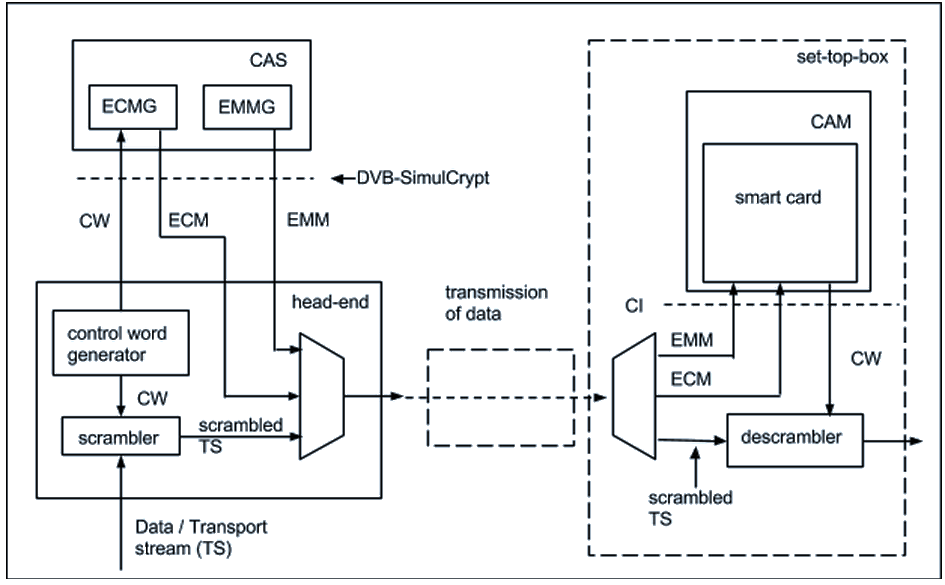
\includegraphics[width=\textwidth]{system}
  \caption{The DVB setup}
  \label{fig:system}
\end{figure}

\section{Head-end} \label{sec:HE}
The head-end is the system where the scrambler is located. Except for 
the scrambler, decoding and generation of program specific information 
takes place in the head-end. The head-end decodes, encrypts and 
encapsulates data which it has received from content providers, 
before transmitting it.

\section{Control word} \label{sec:setup}
TS packets (Transport Streams), which contain data received from 
distributors, are scrambled using a key which is called a 
control word. Control words are usually changed every 120th second, 
but might be changed more often. Some systems change the control word 
every 10th second. Finding out just one control word has very little 
effect on content theft, since it will only be usable for a few 
seconds before being changed. Because of the high frequency in which 
the control words are changed, one means of security is provided. The 
control words are generated randomly to make sure that consecutive 
control words can not be derived from each other.

The following section describes the setup of the DVB system, which can 
be viewed in figure \ref{fig:system}. The control word is sent to a 
CA system (Conditional Access System) where the control word is 
encrypted as an ECM (Entitlement Control Message). The CA system also 
generates an EMM (Entitlement Management Message) which tells the 
smart card, which is located in the CAM (Conditional Access Module), 
contents the user is allowed access to. This could for instance be 
whether the user has paid to view premium football games or not. The 
ECM and EMM are then sent back to the head-end where they are attached 
to the scrambled TS packet using a multiplexer. This package is sent 
to a receiver, which is usually a TV. The ECM, EMM and TS packet are 
separated when they arrive. The ECM and EMM are sent through a 
CI (Common Interface) to the CAM, where the ECM (encrypted control 
word) is decrypted using a decryption algorithm located on the smart 
card. The resulting control word is then used to descramble the TS 
packet. The TS packet is encrypted once more if the CI is a CI+, 
otherwise it is sent in the clear back to the receiver where the data 
is processed before it is dispatched to the user. The CI and CI+ 
as well as the extra encryption are all discussed in section 
\ref{sec:CI}.

\section{Conditional Access System} \label{sec:CAS}
To make sure that users fulfills a set of criteria, before being 
allowed to access content, \emph{Conditional Access} (CA) is used. 
Conditional Access is provided, based on information about the user, 
in a system seperate from the head-end. Content is first scrambled, 
and decoded in a head-end. The control word, used to scramble the 
data, is sent to the Conditional Access system (CAS) where it is 
encoded. The CA system consists of an EMM-generator (noted as EMMG in 
figure \ref{fig:system}) and an ECM-generator (noted as ECMG in figure 
\ref{fig:system}) among others. An ECM-generator encrypts the control 
word. The algorithms used in the generators differ between CA systems 
and is kept very secret, to make sure that the control word can not be 
stolen during transmission.

The ECM is generated using the control word, while the EMM is 
generated based on subscription- and payment information related to 
the user. The ECM-generators are deterministic, and differ from CAS to 
cas. The EMM can allow things, stretching from allowing a user to 
view a video for a few hours, to access a certain channel for an 
extended period of time. A TV will not display any channels without 
receiving an EMM allowing it to.

An example is that a user needs to pay for TV-services to be able 
to access content. The CAS generates an EMM which tells the smart card 
whether the user is allowed to access the requested material or not. 
The content provider also generates an ECM based on the control word, 
which the smart card decrypts and passes to the descrambler which 
decrypts the video stream. This is done if the EMM allows it.

\subsection{Standards}
Some of the CA systems currently in use are Viaccess, Conax, Irdeto, 
NDS, Strong and NagraVision. The CA systems are paired with 
\emph{Conditional Access Module}s (CAM), which are located in the 
receiver. What CAS / CAM pair depends on the content provider. For 
instance, Conax is used by Com Hem, Viaccess is used by Boxer and 
Strong is used by Canal Digital.

\begin{longtable}{| l | c | c |}
  \hline
  CA system & Used by & Supports CI+ \\ \hline
  
  Viaccess & Boxer, SVT & Yes \\ \hline
  Conax & Com Hem & Yes \\ \hline
  Strong & Canal Digital & Yes \\ \hline
\end{longtable}

\section{DVB-SimulCrypt} \label{sec:Simul}
The control words used during scrambling can be sent to several 
different CA systems at once, resulting in several ECMs. This is 
called DVB-SimulCrypt, which is widespread in Europe. DVB-SimulCrypt 
works as an interface between the head-end and the CA system. 
DVB-SimulCrypt encourages the use of several CA systems at once 
\citep{SimulCrypt:2008}. This is done by sending the same control word 
to many CA systems at the same time, and then allowing them each to 
generate an ECM  based on the control word. The multiplexer in the 
head-end then creates TS packets based on those, since the EMMs 
will determine whether the user is allowed access or not. A 
multiplexer is a basic logic circuit, which merges severals signals 
into a single signal.
%OERHÖRT CHANSAT DETTA JA OKEJ KOLLA ÖVER DET! Allt i detta stycke är chansat.

\section{Common Interface} \label{sec:CI}
The Common Interface is the interface between the CAM and the host 
(Digital TV receiver-decoder). There are currently two versions of 
common interfaces in use, which are the CI and the CI+. The difference 
between them is that the output from the CI is unencrypted, while the 
output from the CI+ is encrypted \citep{CI+:2011}. This means that a 
clear TS packet is sent between the CI and the host, that can be 
copied. The data sent between the CI+ and host can not be copied due 
to it being encrypted, and therefore provides more security for 
content providers \citep{CI:1997}.

\subsection{CI+}
The CI+ realizes the possibility of yet another means of protecting 
content, which is called Content Control (noted as CC in Figure 
\ref{img:CIPlus}). Content control is a way of encrypting the content 
inside of the CAM, connected to the CI+ Module. The key used for the 
content control encryption is paired with the Digital TV Receiver, 
where the TS packet is decrypted before being made available to users. 
The general idea can be viewed in Figure \ref{img:CIPlus}.

\begin{figure}[h!]
  \centering
  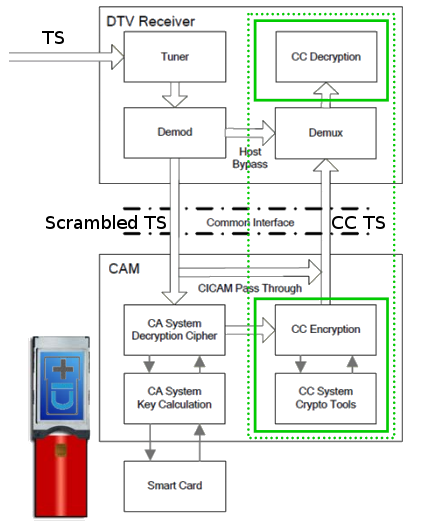
\includegraphics[width=0.7\textwidth]{CIPlus}
  \caption{CI+ interface. \citep[p. 10]{CI+:2011}}
  \label{img:CIPlus}
\end{figure}

CI+ encoding is often used to protect HD content, but not SD 
content. Since HD content is more high-profile, content distributors 
want to protect it more than the SD content. Protection of HD content 
requires scrambling using AES-128 in CBC-mode (explained in section 
\ref{sec:BlockCipher}). \citep{CI+:2011, CI+:2011_2}

\section{Conditional Access Module}\label{sec:CAM}
CA modules (CAMs) are responsible of decoding the scrambled TS packet
received from the host. The CAM is inserted into a PCMCIA slot 
(Personal Computer Memory International Association) either into the 
TV or the set-top box. A set-top box is a box which is connected 
between the TV signal source and the TV. The set-top box is equipped 
with both a CI or CI+, and a CAM. The CAM consists of a slot for a 
smart card and a descrambler. The smart card decodes the ECM and sends 
the control word back to the descrambler. The TS packet is then 
descrambled and the clear data is sent back to the host, from the CAM.

\chapter{Scrambling}\label{ch:Scrambling}
Security is not only about cryptography. But there is a main reason why 
cryptography is attacked , and that is because there is a very low chance 
of being detected. There will be no traces of the attack, since the attacker’s 
access will look just like a legitimate /"good" access. 

This can be compared to a real-life break-in. The break-in will be noticed if 
the thief breaks in using a crowbar. If the thief, on the other hand, would be 
to pick the lock, there is a possibility that you will never notice that your 
security has been breached \citep{Schneier:2003}.

There are many rules concerning cryptography, as there are to all sciences. 
The one I found most noteworthy was that one is to always assume that someone 
is "out to get you". Because of this, \citet[pp. 12--14]{Schneier:2003} say that 
we always need  to look for possible ways to break systems, to make sure that
we are safe.

\section{What is the need for cryptography?}
If we communicate without encrypting the data we are sending, someone 
else will most likely be eavesdropping. For most people this isn’t a problem, 
but in some instances sending secure messages can be extremely important. One 
example is communication during war, where a single piece of intelligence might 
turn the tide of the entire war. Another example is sending manuscripts, and 
drafts of books over the internet. These are some of the reasons as to why we 
want to encode messages.

Another reason for scrambling is to reduce the number of adjacent data-bits with 
the same value, as in long strings of zeros or ones. 

%Balancing the amount of 
%zeros and ones gives a DC balance, which means that the signal is stronger when 
%sent.

\section{Scrambling or Encrypting}
The difference between scrambling and encryption is that scrambling is the
way we generate the secret control word (key) which is used when we make the
data unreadable to outsiders while encryption is the way we protect the control 
word during transmission.

\Warning[Todo]{Det här måste jag bli säkrare på}
% What is the difference between scrambling and encryption? 

\section{Data packets}\label{sec:Data}
The data processed by the DVB systems is sent in data packets. All of them are 
created from ES packets (elementary streams) which generally is the output from 
an audio or video encoder. The ES packets are then packeted into PS, TS or PES 
packets and then distributed. There are three different ways of packing data, 
but only two of them are commonly used. The types are called TS, PS and PES. PS 
packets are used while data isbeing stored, while TS and PES are used when data 
is being transmitted. The ones interresting when working with DVB are therefore 
the TS packets as well as the PES packets.

\subsection{TS packets}
TS packets are the ones used by the DVB society, possibly due to their fixed 
lenghts. TS packets have got a length of 188 bytes with a 4 byte long header, 
meaning the payload consists of 184 bytes. The layout of a TS packet can be 
viewed in figure \ref{img:Package}.

\begin{figure}
  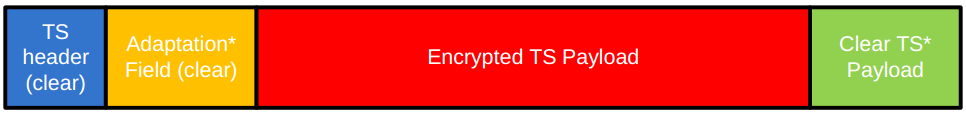
\includegraphics[width=\textwidth]{TSpacket}
  \caption{General layout of a data packet \citep{DVB:2013}}
  \label{img:Package}
\end{figure}

The building blocks that the TS packets consist of are:

\begin{itemize}
\item Header
\item Adaptation field - might not exist
\item Encrypted payload - might not exist
\item Clear payload
\end{itemize}

The header consist of information regarding the packet. The header provides 
information as to whether there is an adaptation field in the packet, what id 
the packet has, the sync byte and two bits telling us whether the data is 
scrambled using an odd or even key, if it is scrambled. The header is never to 
be encrypted and is always found in the beginning of the packets.

The adaptation field is a padding that you input when the end of the data is not 
aligned with the end of the TS packet. This is done to make sure that the TS 
packet is filled. We only find adaptation fields we are working with the last 
string of data, if the data does not align. Adaptation fields are not encrypted.

We are prone to end up with clear bytes of data in the TS packets when we work 
with block ciphers, since block ciphers only encrypt fixed sizes of data. The 
clear data is always located at the end of the packets and can in a worst case 
scenario be up to one byte smaller than the block size, since that will be the 
largest amount of bytes that does not fill an entire block. The encrypted 
payload is always located in front of the clear payload 
\cite[pp. 10--11]{DVB:2013}.

\subsection{PES packets}
The PES packets have varying lengths of up to 64 KBytes.

PES-packets can be of any size less than 64 Kbytes. They are often packed into 
TS packets when distributed, due to the strength of the TS packets. The payload
data in the TS packets consists of the entire PES packets, which consists of the 
header and the data. PES packets do not use adaptation fields, since they can be 
of more or less any length, as long as the packet do not exceed 64 KBytes.

\begin{figure}
  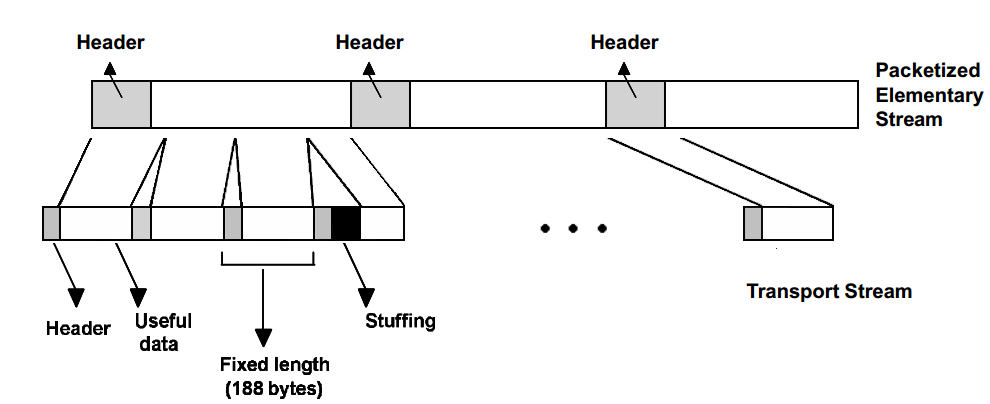
\includegraphics[width=\textwidth]{PES.png}
  \label{img:PES}
  \caption{PES packet derived from TS packets (inspiration for the image 
taken from \citep[p. 9]{ETR:289} ) }
\end{figure}

\section{Encryption and Decryption}
There are two things that you need when you encrypt and decrypt messages. Those 
are the algorithm as well as the key. There are plenty of ways to encrypt 
messages, but there are two ways of sharing the encryption-key. The first method 
being the symmetric-key encryption, and the second method being the public-key 
encryption.

\subsection{Symmetric-key encryption}
The symmetric-key encryption uses the same key to encode and decode messages. 
Distrubution of the key, when using the symmetric-key encryption is troublesome 
and the fact that both parties need access to the same secret key is a major 
drawback of the symmetric key encryption, as compared to the public-key 
encryption method. Sending the key in an email is a bad idea, since the persons 
who wants to read our messages  most likely already will be listening, and they 
will therefore obtain the key as well as the means to decode the messages we 
send.

\subsection{Public-key encryption}
The public-key encryption uses a public key that anyone can look up, and a 
secret key that only one person knows \citep[pp. 25--32]{Simmons:1992}.
For instance say that the two persons, Bob and Alice, want to communicate. 
Bob produces a keypair \(P_{Bob}\) (Bob’s public key) and \(S_{Bob}\) 
(Bob’s secret key) and publishes \(P_{Bob}\) for anyone to see. When Alice wants 
to send Bob a message, she looks up Bob’s public key \(P_{Bob}\), which she then 
uses to encode her message. When she sends Bob the message, Bob decodes the 
message using his secret key \(S_{Bob}\) \citep{Schneier:2003}.

\subsection{Combination}
The big question now is why we would use anything other than the public-key
encryption, since it seems secure and easy to manage. The reason is that the 
public-key encryption is not as effective as the symmetric-key encryption. 
It is common to use a combination of those two since an easy and effective way 
to encrypt messages is what we desire. To do this we use a symmetric-key 
algorithm to encode the plaintext into ciphertext, and then we use the 
public-key encryption to encode the symmteric-key we used when encoding the 
plaintext. This encoded key is then sent together with the ciphertext to the 
recipient, who uses the secret key to decode the symmetric key, which is then used to decipher ciphertext and obtain the plaintext.

Decryption is often performed by reversing the encryption. You need to know the 
algorithm, preferably through a mathematical representation, to calculate how 
to obtain the plaintext from the ciphertext. A description of how this is done 
for the CBC-mode (described in \ref{sec:BlockCipher}) is described in 
\ref{sec:CBCcalc} in appendix \ref{app:misc}. We assume that we know the 
decryption algorithm here for simplicity. \Warning[Source]{feels like a given, but still}

\section{Ciphers}
A cipher is the same as an algorithm, that operates on either plaintexts or 
ciphertexts to perform encryption or decryption. Figure \ref{img:ciphers} 
describes how they can be split into smaller groups.

\begin{figure}
  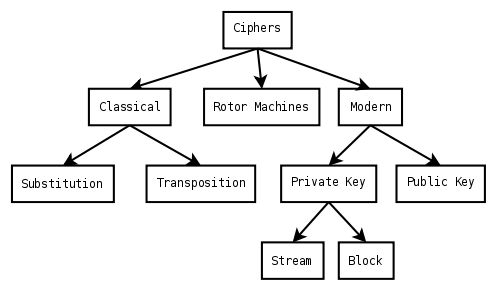
\includegraphics[width=\textwidth]{cipher.png}
  \caption{Different kinds of ciphers \citep{CipherTax:2013}}
  \label{img:ciphers}
\end{figure}

There are mainly two kinds of ciphers that are used when designing modern 
cryptosystems. Those ciphers are called block ciphers and stream ciphers. 
Many systems use a combination of block ciphers and stream ciphers to provide 
security. 
\Warning[Source]{At least the CSA uses it. But you need a source if you want 
this to be here}

\subsection{Block cipher}\label{sec:BlockCipher}
A block cipher operates on blocks where each block consists of a fixed number 
of bytes. This might cause a need for padding the blocks, in case the plaintext 
contains a number of bytes that is not even with the blocksize. Block cipher 
often use itself of a combination of S-boxes and P-boxes in a so-called 
SP-network (Figure \ref{img:SPNetwork}).

There are many modes of block ciphers, but the two recommended by 
\citet{Schneier:2003} are the CBC-mode and the CTR-mode.

CBC stands for \emph{cipher block chaining} and is performed by first encrypting 
the result of an XOR between an IV and the plaintext. This is the ciphertext 
that corresponds to the first plaintext. This is then put into an XOR with the 
next plaintext, and then encrypted \citep[pp. 109--111]{Stinson:2006}. For 
reference, see image \ref{img:CBCmode} in appendix \ref{app:misc}.

CTR stands for \emph{counter}, and refers to the way the IV is generated. The
counter outputs a value, which is encoded with the key. The output is then run 
in an XOR together with the plaintext, producing the ciphertext. The counter is 
then incremented and the procedure is iterated \citep[p. 111]{Stinson:2006}.

\subsection{Stream cipher} \label{sec:StreamCipher}
Stream ciphers work on a stream of data (as implied by the name). They usually 
consist of some kind of a keystream generator which performs a modulo 2 addition
with the data \cite[pp. 67]{Simmons:1992}. An effective implementation of the 
stream cipher is to use a linear feedback shift-register which uses the current 
internal state (key) to produce the next state by a simple XOR-addition between 
two or more of the bits in the state. This is mainly used because of how easy
it is to construct in hardware \citep{LFSR:2008}.

%\citet[{Simmons:1992} claims that there are four main approaches to constructing a stream-cipher; The information-theoretic approach, the system-theoretic approach, the complexity-theoretic approach and randomized stream ciphers.

\section{Confusion and Diffusion}\label{ch:ConfDiff}
Two properties that are needed to ensure that a cipher provides security are 
confusion and diffusion \citep{Shannon:1949}. Note that a cipher is not secure 
just because these two properties are obtained.

\emph{Confusion} refers to making the relationship between ciphertext and key as 
complex as possible. \emph{Diffusion} refers to replacing and shuffling the 
data, to make it impossible to analyze data statistically. This is usually done 
by performing substitutions and permutations in a simple pattern multiple times. 
This can easily be done by using an SP-network (S-box / P-box network) 
\citep[pp. 74--79]{Stinson:2006}. The very first, as well as last step, of 
SP-Networks is usually an XOR between the subkey and the data. This is called 
\emph{whitening}, and is according to \citet[p. 75]{Stinson:2006} regarded as a 
very effective way to prevent encryption/decryption without a known key. 
The goal of this is to make it hard to find the key, even though one has access 
to multiple plaintext/ciphertext pairs produced with the same key 
\citep{Shannon:1949}.

\subsection{S-boxes}
The S-box is one of the basic components that is used when creating ciphers. 
An S-box takes a number of input bits and creates a number of output bits in 
a non-linear fashion \citep[pp. 74--75]{Stinson:2006}. They can effectively be 
implemented as lookup tables. Each input has to correspond to a unique output, 
to make sure that the input can be recreated in the descrambler.

%One way of making it harder to find the relation between the input and the output is to place adjacent bits far from each other in the lookup table 
\Warning[TODO]{You need sources for this!}. 

% CONFUSION OR DIFFUSION?

\subsection{P-Boxes}
The second basic component used in cryptography is the P-box. A P-box 
shuffles/rearranges the order of given bits. This can be viewed in the 
SP-network in figure \ref{img:SPNetwork}, where the P-box is represented by the 
dotted rectangle in the middle.

\begin{figure}
  \begin{center}
    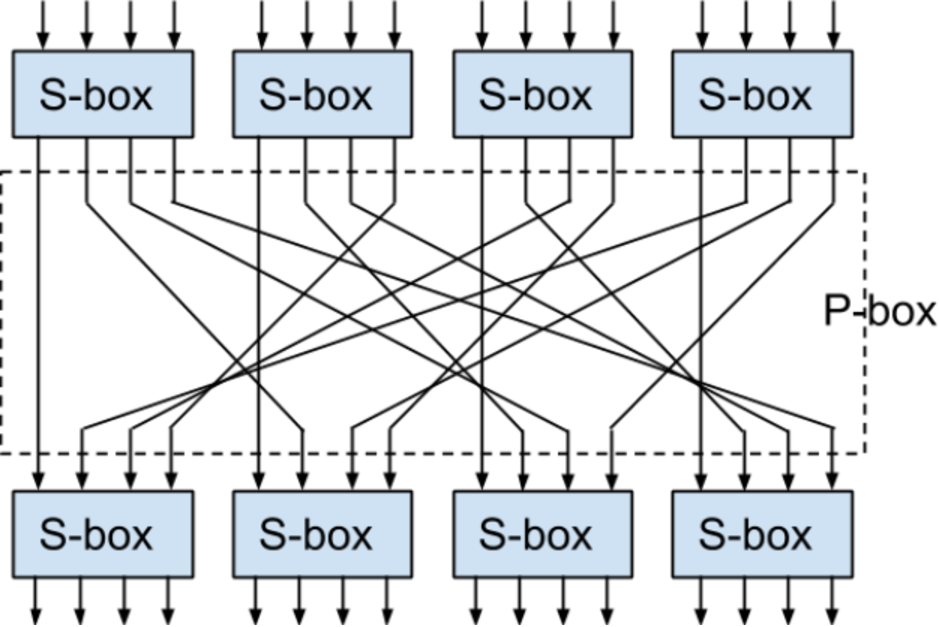
\includegraphics[width=0.8\textwidth]{SPnetwork}
    \caption{SP-Network}
    \label{img:SPNetwork}
  \end{center}
\end{figure}

%CONFUSION OR DIFFUSION?

\section{Secrecy}
Although encryption is important, as well as the strength of the encryption, 
keeping the algorithm secret is never a good idea. A simple mistake when 
designing an algorithm might turn an encryption that would have been strong,
incredibly weak. It is therefore a bad idea to use small scale algorithms  
(designed for the use of just a few persons for instance). If you instead 
use an open algorithm, faults will most likely be discovered and fixed by 
experienced cryptographers \citep[pp. 23]{Schneier:2003}. Keeping the key, 
which is used to encrypt the data, secret is what is important.

\chapter{CSA} \label{ch:CSA}
The CSA is currently the most commonly used encryption algorithm in DVB for 
encryption of video-streams. There are two versions of the DVB-CSA, CSA1 and 
CSA2. The only difference between them being the key-length 
\citep[p. 23]{DVBScene:2013}. The CSA uses a combination of a block cipher 
taking an input of a 64-bit block, and a stream cipher. Both of the ciphers use 
the same key, so that the entire system uses the same key 
\citep[pp. 271--272]{WeiLi:2007}. This means that the complete algorithm would 
break if the key would be recovered. Using the same key does on the other hand 
allow us to change the key at regular intervals more easily. 

CSA has been the official scrambling method for DVB since may 1994. CSA was 
to be implemented in hardware and hard to implement in software, for the sake
 of making reverse-engineering difficult \citep{DVBScene:2013}.

\section{History} \label{sec:History}
CSA was largely kept secret until 2002. It was made very hard to reverse engineer
since it was largely implemented in hardware. The patent papers gave some hints
of the layout, but important details like the layout of the S-boxes remained 
secret.
Without the S-boxes, free implementations of the algorithm were out of question. 
Initially, CSA was to remain implemented in hardware only, but software 
implementations were found on the internet, which made it possible to analyze
the entire solution.

In 2002 FreeDec was released, implementing CSA in software. Though released as 
binary only, disassembly revealed the missing details and allowed 
reimplementation of the algorithm in higher-level programming languages. 
\Warning[source]{Is this relevant, and you need another source than Wikipedia}

With CSA now publicly known in its entirety, cryptanalysts started looking for 
weaknesses.

\begin{figure}
  \begin{center}
    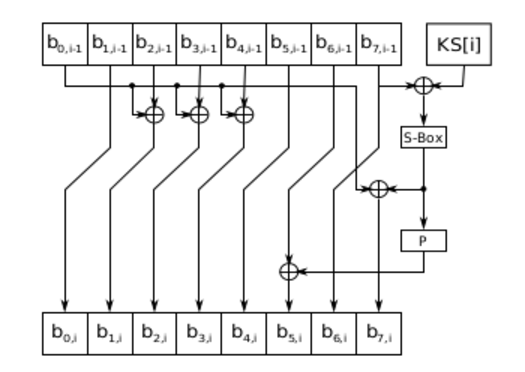
\includegraphics{blockcipher}
  \end{center}
  \caption{Image from \citet[pp. 49]{Breaking:2012}}
  \label{fig:blockcipher}
\end{figure}

\section{Layout of the CSA}
The CSA consists a block cipher and a stream cipher connected in sequence 
\citep[p. 271]{WeiLi:2007}. The block cipher reads 64-bit blocks of data, which 
is then run in an CBC-mode. The block cipher processes these blocks of data in 
56 rounds. The output of this is sent to the stream cipher where additional 
encoding is performed. The first block of data sent from the block cipher to the 
stream cipher is used as an IV for the stream cipher, and is not encoded in this 
phase. \citep{DVBAnalysis:2006}

\section{Breaking the CSA}
There are a few standard ways to try when you want to break a cipher. 
Those are the brute force approach, known-plaintext attacks, chosen plaintext 
attacks and birthday attacks \citep[pp. 31-34]{Schneier:2003}. You choose what 
method to use depending on what the ciphers look like. I will not discuss all 
of them, but I will talk about the most relevant ones here.

\subsection{CW sharing}
One of the problems with the CW distribution is the fact that CW sharing has 
become a real problem \citep{Farncombe}. This is possible due to the fact that
the CW is sent in the clear between the smart card and the STB, meaning that a 
user might grab the clear CW and redistribute it over the internet. 
This has become a financial problem for content distributors, since people stop 
paying for the content which they are watching.

One way of dealing with CW sharing is to decode the encrypted CW on the CI 
system, and then encrypt it once again on the CI, before sending it to the STB. 
The latter key is setup between the CI system and the STB  through a one time
sychronization. This means that users are not able to grab the clear CW and 
redistribute it. \citep[pp. 12--13]{HIS:2011}

\hrulefill
\hrule
Nu ska jag försöka få in att man inte får lägga TS streams i översta lagret, så 
att folk kan koppla in hårdvara och försöka sno data från översta lagret. Det 
finns därmed väldigt mycket krav på hur hårdvaran ser ut.
\hrulefill
\hrule

\subsection{Brute force}
The CSA uses a key consisting of 64-bits, which gives us 18.5 Quintillion 
possible keys (Quintillion is $10^{18}$). But byte 3 and 7 are often used as 
parity bytes in CA systems which leads to only 48 bits being used in the key 
\citep{Breaking:2012}. This can be seen in figure \ref{fig:blockcipher}. 48 bits 
on other hand leads to $2^{48}$ combinations, which corresponds to 281 trillion 
possible keys (Trillion is $10^{12}$). Testing a million keys per second is about 
what is possible through on a modern x86 processor using software methods
\Warning[Todo]{How did I get this number?}, which means it would take roughly 
3258 days to force brake the keys. That is roughly 8.8 years.

Moreover, systems need to change the key at least every 120 seconds \citep{Simpson:2009} and most systems issues new keys every 10-120 second \citep{Wirt:2004}.

It is possible to use dedicated hardware and FPGA implementations to speed this 
up, using hardware accelerations and other methods. But even if we would then 
be able to scan through 2.8 trillion keys per second, precisely allowing us to 
be certain to find the key in two minutes, we could just change the key more 
often. As such, the brute force method of obtaining the key is not an option.

%\subsection{Bit slicing}
%The stream cipher part of CSA is prone to bit slicing, a software implementation 
%technique that allows decryption of many blocks, or the same block with many 
%different keys, at the same time. This significantly speeds up a brute force 
%search implemented in software, although the factor is too low to make a real-time 
%attack practical.

%The block cipher part is harder to bit slice, as the S-boxes involved are too large 
%(8x8) to be efficiently implemented using logical operations, a prerequisite for bit 
%slicing to be more efficient than a regular implementation.

\section{Why do we need a new standard?}
The DVB-CSA standard offers short-term protection (it assumed content is viewed 
in real time and not stored). But due to the development during recent years, 
we now need to be able to distribute the content around the home. This means 
that the focus needs to be moved from securing the delivery, to securing the 
content. \citep{Farncombe}


There are currently two implementations suggested for doing this. The first is 
the hardware friendly CSA3 which uses itself of AES blocks (with keys of sized 
128, 192 or 256 bits) as well as a confidential block cipher called the XRC. The 
second version is the software friendly CISSA which uses the AES-128 as a basic 
building block. \citep{DVB:2013}

What are the pros and cons of having hardware scramblers and software scramblers.
Software uses itself of the date to generate a random key. Hardware uses itself 
of additive scramblers, and other random output generators to generate the key. 


\chapter{CISSA and CSA3}
There are currently two scrambling algorithms being assessed as replacements to 
the currently used DVB-CSA. This is done to assure content security for 
yet another ten years.

%%%%%%%%%%%%%%
%What are the pros and cons of having hardware scramblers and software scramblers.Software uses itself of the date to generate a random key. Hardware uses itself %of additive scramblers, and other random output generators to generate the key. %%%%%%%%%%%%%%

CISSA is meant to be a hardware-friendly as well as software-friendly algorithm 
designed to allow descrambling on CPU-based units such as computers, smart phones
and tablets \citep[p. 9]{DVB:2013}. CISSA 

CSA3 is a hardware-friendly, software-unfriendly scrambling algorithm chosen by 
the ETSI to replace the currently used CSA \citep[pp. 6--7]{DVB:2013}. It uses 
itself of AES blocks (with keys of lengths of either 128, 192 or 256 bits) as 
well as a confidential block cipher called the XRC for scrambling. 
Software-unfriendly means that descrambling is designed so that it is highly 
impractical to perform in software, but is easily done in hardware.

Both of the algorithms are to be implemented in hardware for scrambling of data.
The difference is that CSA3 is to make it hard to descramble the material in 
software. Since both of the algorithms are confidential, it is sadly impossible 
to find out what makes the CSA3 algorithm software-unfriendly, while the CISSA 
algorithm is software-friendly. \Warning[Source]{Om jag får be snällt}

\section{CISSA}
CISSA stands for \emph{Common IPTV Software-oriented Scrambling Algorithm} and 
is designed to be software-friendly. Opposite to the CSA3, CISSA is made to be 
easily descrambled in software, so that CPU-based systems such as computers and 
smart-phones can also implement it.  Although it is software-friendly, it is 
supposed to able to be implemented efficiently on hardware as well as in 
software \citep[p. 9]{DVB:2013}.

CISSA is to use the AES-128 block cipher in CBC-mode with a 16 byte IV with the 
value 0x445642544d4350544145534349535341. \citep[p. 11]{DVB:2013}

Är inte meningen att ens IV ska vara hemlig? Den utgör ju en stor del an shiffret? Om man vet IV borde man kunna inputta en ciphertext som plaintext så att man kan ta reda på vilken det ursprungliga plaintexten var?
\Warning[Find more]{But I don't know the name of the second block cipher}

\subsection{Software friendly}
What makes this algorithm software friendly?
Is it still possible to make use of it on an FPGA - since FPGAs are so
general?

\section{CSA3}
CSA is to be succeeded by CSA3 which is based on a combination of a 128-bit 
AES block cipher, which is simply called the AES-128, and a confidential block 
cipher called the XRC \citep[p. 8]{DVB:2013}.

\subsection{XRC}
XRC stands for eXtended emulation Resistant Cipher and is a confidential cipher 
used in DVB \citep[p. 8]{DVB:2013}.

\subsection{Hardware friendly}
What makes the CSA3 so hardware friendly?
Is it because it is meant to be a secret standard, only to be delivered
on a chip, to make it as good as impossible to reverse-engineer?

\section{Conclusion}
From what I've seenff, both the CISSA and CSA3 implement the AES-128 for 
scrambling, combined with a secret cipher. The secret cipher for CSA3 is the XRC 
cipher, and the secret CISSA cipher is yet to be known FÖR JAG HAR INTE HITTAT DET, MEN DET BETYDER INTE ATT ANDRA INTE VET VAD DET HETER. CISSA sounds like a 
great idea in my opinion, allowing CPU-based units to descramble data streams 
without a dedicated HW-Chip. While that is good and all, CSA3 is a finished 
standard, and will probably be more easily implemented on an FPGA, while CISSA 
seems to be still developed. Starting out with an AES-128 chiper would provide 
for a basis to continue development of the scrambling, either towards the CISSA 
or the CSA3 solution, on a later stage.

\chapter{Advanced Encryption Standard}\label{ch:AES}
Both CSA3 and CISSA use the block cipher called AES, which will be 
explained in this chapter. The standard was determined by NIST in 
November 2001. AES is a symmetric block cipher which uses itself of
key lengths of either 128, 192 or 256 bits. It is based on an 
SP-network which is fast in both hardware and software. 

\section{Introduction}
The Rijndael cipher, which is used in AES, has key-sizes of at least 
128 bits. The block length is 128 bits. It uses 8 to 8 bit S-boxes 
and a encryption is made with a minimum of 10 rounds of repetition 
\citep[p. 79]{Stinson:2006}. A round can corresponds to one iteration 
of a certain part of the algorithm, and uses a subkey to the provided 
key. The keys used in the rounds are called round keys. It is a 
symmetric-key algorithm with a fixed block size of 128 bits, where the 
key-size can vary between 128, 192 or 256 bits. The number of cycles 
needed to convert the plaintext into ciphertext depends on the size of 
the key. The 128-bit key requires 10 cycles of repetitions (rounds). 
The 192-bit key requires 12 rounds and the 256-bit key requires 14 
rounds. \citep[p. 103]{Stinson:2006}

\section{Method}
The AES consists of a number of steps that are repeated for each block 
to be encoded. All of the steps are explained later in this chapter.
The steps to be performed are, according to \citet{Stinson:2006}:

\emph{Set-up steps}
\begin{enumerate}
\item KeyExpansion - Produce round keys.
\item InitialRound - Combine each byte of the state with a byte of 
  round key.
\end{enumerate}
\emph{Steps performed during the rounds}
\begin{enumerate}
\item SubBytes - Each byte is \emph{substituted} using the Rijndael's 
  S-box.
\item ShiftRows - The rows of the state matrix are \emph{permutated}.
\item MixColums - The columns of the state matrix are multiplicated with a 
  matrix.
\item AddRoundKey - The state matrix is once again combined with 
  round-keys.
\end{enumerate}
\emph{In the final round everything except the MixColumns step are 
performed. Meaning that SubBytes, ShiftRows and AddRoundKey are 
performed.}

The ciphertext is then defined as the state-matrix 
\citep[p. 103]{Stinson:2006}. As mentioned in section 
\ref{ch:ConfDiff} (\nameref{ch:ConfDiff}), both confusion and 
diffusion are nescessary to ensure a secure encryption. They can be 
seen in the SubBytes and ShiftRows steps above. These steps also 
performs whitening, which strengthens the cipher. Whitening is, as 
mentioned in \ref{ch:ConfDiff}, performed through an XOR between the 
roundkey and the data.

The KeyExpansion is explained in section \ref{sec:KeySch}.

Before anything can be done, the data needs to be put into a 
state-matrix, which can be seen in figure \ref{matrix2:state}.

\begin{figure}[h!]
  \begin{equation}
    \begin{bmatrix}
      a_{1, 1} & a_{1, 2} & a_{1, 3} & a_{1, 4} \\
      a_{2, 1} & a_{2, 2} & a_{2, 3} & a_{2, 4} \\
      a_{3, 1} & a_{3, 2} & a_{3, 3} & a_{3, 4} \\
      a_{4, 1} & a_{4, 2} & a_{4, 3} & a_{4, 4}
    \end{bmatrix}
  \end{equation}
  \caption{State-Matrix}
  \label{matrix2:state}
\end{figure}

\subsection{InitialRound}
This is an initial AddRoundKey which is explained in section 
\ref{sec:AddRoundKey}.

\subsection{SubBytes}
In the SubBytes step, each byte is sent to a Rijndael S-box (which is 
basically a lookup table, see figure \ref{matrix:rijSbox} in appendix 
\ref{app:matrix}) where they are substituted in a non-linear fashion. 
This gives us a substituted state matrix.

\subsection{ShiftRows}
The next step is called the ShiftRows step, which left-shifts the rows 
n-1 steps where n is the index of the row. This means that the first 
row is left as it is, the second row is shifted one step, the third 
row is shifted two steps, and the fourth row is shifted three steps.
The data is shifted cyclically, meaning that data which is shifted 
out of the left side of the state-matrix is shifted back in from the 
right side.

\subsection{MixColumns}
All of the multiplications performed in the MixColumns steps are 
take place in the Galois Field, which is why a lot of it might seem
illogical at first. 

In the MixColumns step, the four bytes of each row are combined 
through a matrix multiplication. The MixColumns function takes four 
bytes as input and multiplies them with a fixed matrix (figure 
\ref{matrix:rijMix} in appendix \ref{app:matrix}). While this might 
seem simple to do, it actually is not. The multiplication makes sure 
that each input byte affect all output bytes. \citep{Angelfire}

The matrix is multiplicated with the vector from the left, (4x4*4x1 = 
4x\hcancel{4*4x}1 = 4x1) where the vector is a column from the 
state-matrix. Multiplication with 1 means that the value is left 
untouched. Multiplication by 2 means left shift, then an XOR with 0x1B 
if the shifted value exceeds 0xFF. Multiplication with 3 is done in 
the same way as a multiplication with 2, except that the result after 
the shift and conditional XOR are then XOR:ed with the input value of 
the multiplication. All of the resulting values are then XOR:ed, 
leaving us with the result. All additions are replaced with XOR, since 
the calculations take place in the Galois Field (GF(\(2^8\))).

\subsection{AddRoundKey}\label{sec:AddRoundKey}
Each of the 16 bytes of the state are combined with a byte from the 
round key using a bitwise XOR. They are then combined to a state 
matrix (Figure \ref{matrix:state} in Appendix \ref{app:matrix}) 
containing 4x4 bytes.

\section{KeyExpansion}\label{sec:KeySch}
To generate round keys from the provided key, the Rijndael's key 
schedule is used. The schedule consists of a couple of loops and a key-
schedule core. The schedule core is the part that branches out if c 
modulo 16 is zero. The flowchart explaining the entire KeyExpansion 
can be viewed in Figure \ref{img:keysch} in Appendix \ref{app:fig}. 
To change the key schedule to fit a key size of 192 bits, you simply 
change the value that c is compared to in the first branch in the 
flowchart from 176 to 206.

This is done since AES requires a separate 128-bit (16-byte) 
round key for each round, plus one extra key for the initialization 
which means that the AES-128 requires 176 bytes, since AES-128 consists
of 10 rounds.

\subsection{Key-schedule core}\label{sec:kCore}
The key-schedule core takes an input of 4 bytes (32 bits) which it 
then rotates 1 byte (8 bits) to the left. Let us say that our key is 
\emph{AB CD EF 01}. This would give us the key \emph{CD EF 01 AB} 
after the rotation. This operation is also called the RotWord-
operation \citep[p. 107]{Stinson:2006}. The next step is to apply 
Rijndael's S-box to each of these bytes, giving us 4 new bytes. The 
bytes {AB CD EF 01} would give us {62 BD DF 7C}, when substituted 
according to the Rijndael S-box (Figure \ref{matrix:rijSbox} in 
Appendix \ref{app:matrix}).

The left-most byte is then XOR:ed with a value from the Rcon function 
depending on what round you are currently processing. You can read 
more about the Rcon function in section \ref{ch:Rcon}.

\subsection{Rijndael's S-Box}
Rijndael's S-box takes an input byte which it transforms according to 
a LUT (Figure \ref{matrix:rijSbox} in Appendix \ref{app:matrix}). 
Where the most significant nibble is located on the Y axis, and the 
least significant nibble is located on the X axis of the table. Given 
the input \emph{0x31}, the output \emph{0xC7} would be received from 
the Rijndael's S-box.

\subsection{Rcon} \label{ch:Rcon}
The value input into the Rcon function depends on what round you are 
currently at. Which means that you would choose Rcon(1) for the first 
round, Rcon(2) for the second round, and so on. The values in the Rcon 
array are calculated mathematically, but might as well be accessed 
from a vector, such as the one found in Figure \ref{matrix:rcon} in 
Appendix \ref{app:matrix}.

The steps to be performed in the Rcon function are illustrated in a
flowchard and can be viewed in figure \ref{img:rcon} in appendix 
\ref{app:fig}.

If the input value is 0, the output value is 0, otherwise the 
following steps are performed \citep{RijndaelKeySchedule}. This can 
also be replaced by an S-box where you input your byte, and get 
another back, since the input byte is just used as a counter that 
decides how many times you perform steps \ref{item:step1} through 
\ref{item:step3} 

\begin{enumerate}
\item Set a variable c to 0x01.
\item If the input-value does not equal 1, set variable b to c 
  \& 0x80. Otherwise, go to \ref{item:exit_loop}. 
  \label{item:step1}
\item Left shift c one step.
\item If b is equal to 0x80 proceed to \ref{item:step2}, otherwise go to
  \ref{item:step3}.
\item Store the result of a bitwise XOR between c and 0x1B in c.
  \label{item:step2}
\item Decrease the input value by one, then go back to  
  \ref{item:step1}.
  \label{item:step3}
\item The output is set to c.
  \label{item:exit_loop}
\end{enumerate}


\chapter{Result}
Här är väl tanken att jag ska skriva lite om hur jag implementerat
och bearbetat allt relevant som har med implementationen att göra. 
Vad jag gjort som blivit bättre än andra lösningar. Vad jag fokuserat
 på (throughput kontra mängd använd hårdvara).

\section{Problems}
Encountered problems:

\begin{itemize}
\item Not possible to get the license for CSA3
\item Small interrest for CSA3
\item Next to no documentation of the CISSA algorithm
\end{itemize}

% Fortsätt fylla i när du stöter på problem

\section{Hardware}
Såhär ser hårdvaran ut i en sjukt snygg bild jag ritat: \newline

\begin{array}{r l c r l}
  Inputs & &  \_\_\_\_\_\_\_ & & Outputs \\
  1 & --| & & | -- & 1 \\
  2 & --| & & | -- & 2 \\
  3 & --| & HW & | -- & 3 \\
  4 & --| & & | -- & 4 \\
  5 & --| & & | -- & 5 \\
  &     &   \_\_\_\_\_\_\_ & & \\
\end{array}

\section{Flow}
Berätta om flödet på implementationen.

\section{Special solutions}
Berätta om hur det fungerar.

\section{How much of the CSA3 standard has been implemented?}
Berätta om vilka delar du realiserat.


\part*{Appendix}
\appendix

\chapter*{Matrixes} \label{app:matrix}

\arraycolsep=3pt

\begin{figure}
  \begin{equation}
    \begin{array}{c | c c c c c c c c c c c c c c c c}
      Nibble	& 00 & 01 & 02 & 03 & 04 & 05 & 06 & 07 & 08 & 09 & 0A 
      & 0B & 0C & 0D & 0E & 0F \\ \hline
      00		& 63 & 7C & 77 & 7B & F2 & 6B & 6F & C5 & 30 
      & 01 & 67 & 2B & FE & D7 & AB & 76 \\
      10		& CA & 82 & C9 & 7D & FA & 59 & 47 & F0 & AD 
      & D4 & A2 & AF & 9C & A4 & 72 & C0 \\
      20		& B7 & FD & 93 & 26 & 36 & 3F & F7 & CC & 34 
      & A5 & E5 & F1 & 71 & D8 & 31 & 15 \\
      30		& 04 & C7 & 23 & C3 & 18 & 96 & 05 & 9A & 07 
      & 12 & 80 & E2 & EB & 27 & B2 & 75 \\
      40		& 09 & 83 & 2C & 1A & 1B & 6E & 5A & A0 & 52 
      & 3B & D6 & B3 & 29 & E3 & 2F & 84 \\
      50		& 53 & D1 & 00 & ED & 20 & FC & B1 & 5B & 6A 
      & CB & BE & 39 & 4A & 4C & 58 & CF \\
      60		& D0 & EF & AA & FB & 43 & 4D & 33 & 85 & 45 
      & F9 & 02 & 7F & 50 & 3C & 9F & A8 \\
      70		& 51 & A3 & 40 & 8F & 92 & 9D & 38 & F5 & BC 
      & B6 & DA & 21 & 10 & FF & F3 & D2 \\
      80		& CD & 0C & 13 & EC & 5F & 97 & 44 & 17 & C4 
      & A7 & 7E & 3D & 64 & 5D & 19 & 73 \\
      90		& 60 & 81 & 4F & DC & 22 & 2A & 90 & 88 & 46 
      & EE & B8 & 14 & DE & 5E & 0B & DB \\
      A0		& E0 & 32 & 3A & 0A & 49 & 06 & 24 & 5C & C2 
      & D3 & AC & 62 & 91 & 95 & E4 & 79 \\
      B0		& E7 & C8 & 37 & 6D & 8D & D5 & 4E & A9 & 6C 
      & 56 & F4 & EA & 65 & 7A & AE & 08 \\
      C0		& BA & 78 & 25 & 2E & 1C & A6 & B4 & C6 & E8 
      & DD & 74 & 1F & 4B & BD & 8B & 8A \\
      D0		& 70 & 3E & B5 & 66 & 48 & 03 & F6 & 0E & 61 
      & 35 & 57 & B9 & 86 & C1 & 1D & 9E \\
      E0		& E1 & F8 & 98 & 11 & 69 & D9 & 8E & 94 & 9B 
      & 1E & 87 & E9 & CE & 55 & 28 & DF \\
      F0		& 8C & A1 & 89 & 0D & BF & E6 & 42 & 68 & 41 
      & 99 & 2D & 0F & B0 & 54 & BB & 16
    \end{array}
  \end{equation}
  \caption{Rijndael S-box}
  \label{matrix:rijSbox}
\end{figure}

\begin{figure}
  \begin{equation}
    \begin{bmatrix}
      a_{1, 1} & a_{1, 2} & a_{1, 3} & a_{1, 4} \\
      a_{2, 1} & a_{2, 2} & a_{2, 3} & a_{2, 4} \\
      a_{3, 1} & a_{3, 2} & a_{3, 3} & a_{3, 4} \\
      a_{4, 1} & a_{4, 2} & a_{4, 3} & a_{4, 4}
    \end{bmatrix}
  \end{equation}
  \caption{State-Matrix}
  \label{matrix:state}
\end{figure}

\begin{figure}
  \begin{equation}
    \begin{bmatrix}
      2 & 3 & 1 & 1 \\
      1 & 2 & 3 & 1 \\
      1 & 1 & 2 & 3 \\
      3 & 1 & 1 & 2
    \end{bmatrix}
    \*
    \begin{bmatrix}
      a_{1,i} \\ 
      a_{2,i} \\
      a_{3,i} \\
      a_{4,i}
    \end{bmatrix}
    ,i = \{1,2,3,4\}
  \end{equation}
  \caption{Rijndael MixColumns equation}
  \label{matrix:rijMix}
\end{figure}

\begin{figure}
  \begin{array}{l l l l l l l l l l l l l l l l l}
    Rcon[256]=\{ & 8D & 01 & 02 & 04 & 08 & 10 & 20 & 40 & 80 & 1B & 36 & 6C & D8 & AB & 4D & 9A \\ 
    & 2F & 5E & BC & 63 & C6 & 97 & 35 & 6A & D4 & B3 & 7D & FA & EF & C5 & 91 & 39 \\ 
    & 72 & E4 & D3 & BD & 61 & C2 & 9F & 25 & 4A & 94 & 33 & 66 & CC & 83 & 1D & 3A \\ 
    & 74 & E8 & CB & 8D & 01 & 02 & 04 & 08 & 10 & 20 & 40 & 80 & 1B & 36 & 6C & D8 \\ 
    & AB & 4D & 9A & 2F & 5E & BC & 63 & C6 & 97 & 35 & 6A & D4 & B3 & 7D & FA & EF \\
    & C5 & 91 & 39 & 72 & E4 & D3 & BD & 61 & C2 & 9F & 25 & 4A & 94 & 33 & 66 & CC \\
    & 83 & 1D & 3A & 74 & E8 & CB & 8D & 01 & 02 & 04 & 08 & 10 & 20 & 40 & 80 & 1B \\
    & 36 & 6C & D8 & AB & 4D & 9A & 2F & 5E & BC & 63 & C6 & 97 & 35 & 6A & D4 & B3 \\
    & 7D & FA & EF & C5 & 91 & 39 & 72 & E4 & D3 & BD & 61 & C2 & 9F & 25 & 4A & 94 \\
    & 33 & 66 & CC & 83 & 1D & 3A & 74 & E8 & CB & 8D & 01 & 02 & 04 & 08 & 10 & 20 \\
    & 40 & 80 & 1B & 36 & 6C & D8 & AB & 4D & 9A & 2F & 5E & BC & 63 & C6 & 97 & 35 \\
    & 6A & D4 & B3 & 7D & FA & EF & C5 & 91 & 39 & 72 & E4 & D3 & BD & 61 & C2 & 9F \\
    & 25 & 4A & 94 & 33 & 66 & CC & 83 & 1D & 3A & 74 & E8 & CB & 8D & 01 & 02 & 04 \\
    & 08 & 10 & 20 & 40 & 80 & 1B & 36 & 6C & D8 & AB & 4D & 9A & 2F & 5E & BC & 63 \\
    & C6 & 97 & 35 & 6A & D4 & B3 & 7D & FA & EF & C5 & 91 & 39 & 72 & E4 & D3 & BD \\
    & 61 & C2 & 9F & 25 & 4A & 94 & 33 & 66 & CC & 83 & 1D & 3A & 74 & E8 & CB & 8D\}
  \end{array}
  \caption{The Rcon function represented as a vector}
  \label{matrix:rcon}
\end{figure}


\chapter{Flowcharts} \label{app:fig}
This appendix contains flowcharts that describe the extraction of the 
value from the rcon function, and how to perform a keyexpansion.
They are placed in this appendix instead of the thesis since they 
can be used for reference, but are not nescessary to understand how 
the results are obtained.

\begin{figure}
  \begin{center}
    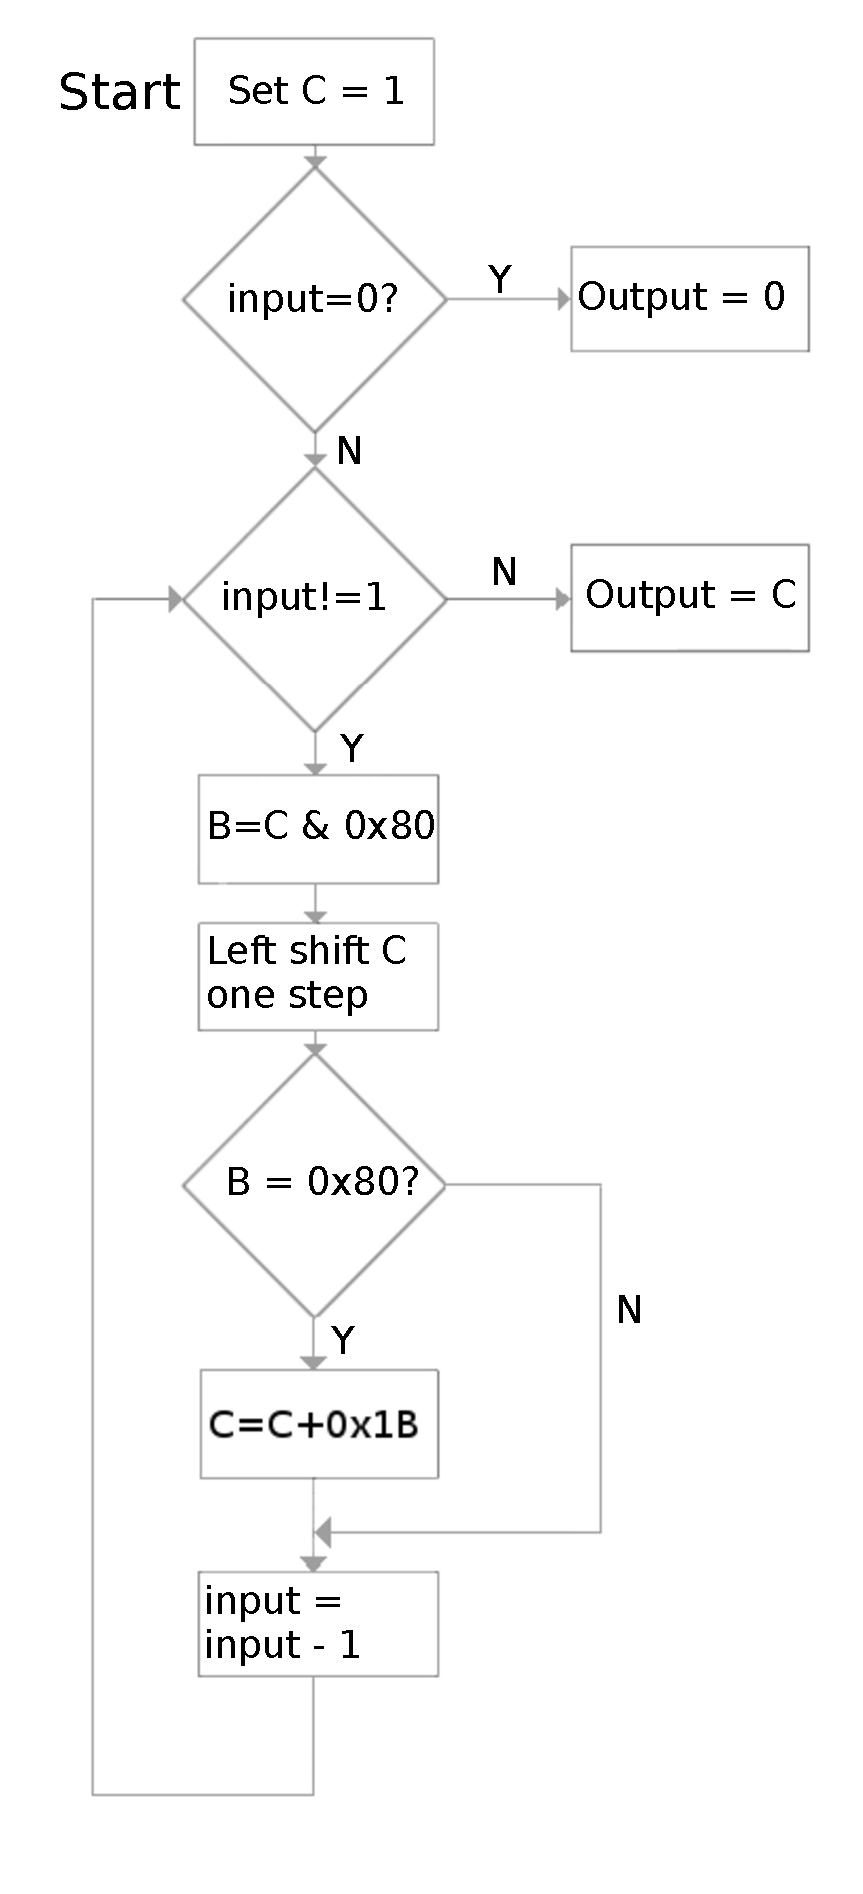
\includegraphics[height=0.6\textheight]{flowchart}
  \end{center}
  \caption{Flowchart of the Rcon function}
  \label{img:rcon}
\end{figure}

\begin{figure}
  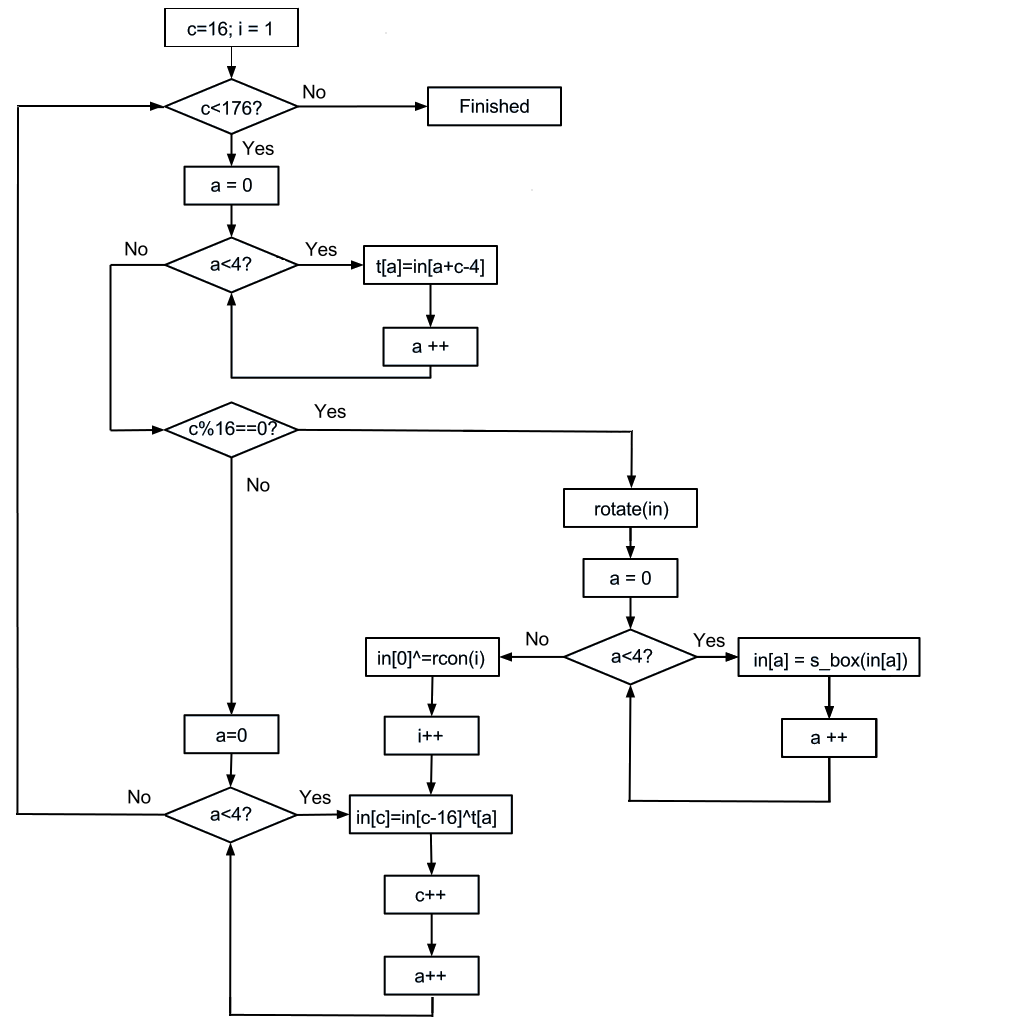
\includegraphics[width=\textwidth]{keyschedule}
  \caption{Flowchart of the key schedule}
  \label{img:keysch}
\end{figure}



\chapter{Test vectors}

\arraycolsep=1pt

\Warning[Todo]{Fixa så det här blir fint}
A.1 Expansion of a 128-bit Cipher Key
This section contains the key expansion of the following cipher key:

Cipher Key = 2b 7e 15 16 28 ae d2 a6 ab f7 15 88 09 cf 4f 3c

for Nk = 4, which results in 
w0 = 2b7e1516 
w1 = 28aed2a6 
w2 = abf71588 
w3 = 09cf4f3ci

\begin{figure}[h]
  \centering
  \begin{array}{| c | c | c | c | c | c | c | c |}
    \hline
    &  & After & After &  & After \oplus &  & w[i] = \\
    i(dec) & temp & RotWord & SubWord & Rcon(i) & with Rcon & w[i-Nk] & temp 
    \oplus w[i-Nk] \\ \hline
    4 & 09cf4f3c & cf4f3c09 & 8a84eb01 & 01000000 & 8b84eb01 & 2b7e1516 & 
    a0fafe17 \\ \hline
    5 & a0fafe17 & & & & & 28aed2a6 & 88542cb1 \\ \hline
    6 & 88542cb1 & & & & & abf71588 & 23a33939 \\ \hline
    7 & 23a33939 & & & & & 09cf4f3c & 2a6c7605 \\ \hline
    8 & 2a6c7605 & 6c76052a & 50386be5 & 02000000 & 52386be5 & a0fafe17 & 
    f2c295f2 \\ \hline
    9 & f2c295f2 & & & & & 88542cb1 & 7a96b943 \\ \hline
    10 & 7a96b943 & & & & & 23a33939 & 5935807a \\ \hline
    11 & 5935807a & & & & & 2a6c7605 & 7359f67f \\ \hline
    12 & 7359f67f & 59f67f73 & cb42d28f & 04000000 & cf42d28f & f2c295f2 & 
    3d80477d \\ \hline
    13 & 3d80477d & & & & & 7a96b943 & 4716fe3e \\ \hline
    14 & 4716fe3e & & & & & 5935807a & 1e237e44 \\ \hline
    15 & 1e237e44 & & & & & 7359f67f & 6d7a883b \\ \hline
    16 & 6d7a883b & 7a883b6d & dac4e23c & 08000000 & d2c4e23c & 3d80477d &
    ef44a541 \\ \hline
    17 & ef44a541 & & & & & 4716fe3e & a8525b7f \\ \hline
    18 & a8525b7f & & & & & 1e237e44 & b671253b \\ \hline
    19 & b671253b & & & & & 6d7a883b & db0bad00 \\ \hline
    20 & db0bad00 & 0bad00db & 2b9563b9 & 10000000 & 3b9563b9 & ef44a541 & 
    d4d1c6f8 \\ \hline
    21 & d4d1c6f8 & & & & & a8525b7f & 7c839d87 \\ \hline
    22 & 7c839d87 & & & & & b671253b & caf2b8bc \\ \hline
    23 & caf2b8bc & & & & & db0bad00 & 11f915bc \\ \hline
    24 & 11f915bc & f915bc11 & 99596582 & 20000000 & b9596582 & d4d1c6f8 & 
    6d88a37a \\ \hline
    25 & 6d88a37a & & & & & 7c839d87 & 110b3efd \\ \hline
    26 & 110b3efd & & & & & caf2b8bc & dbf98641 \\ \hline
    27 & dbf98641 & & & & & 11f915bc & ca0093fd \\ \hline
    28 & ca0093fd & 0093fdca & 63dc5474 & 40000000 & 23dc5474 & 6d88a37a &
    4e54f70e \\ \hline
    29 & 4e54f70e & & & & & 110b3efd & 5f5fc9f3 \\ \hline
    30 & 5f5fc9f3 & & & & & dbf98641 & 84a64fb2 \\ \hline
    31 & 84a64fb2 & & & & & ca0093fd & 4ea6dc4f \\ \hline
    32 & 4ea6dc4f & a6dc4f4e & 2486842f & 80000000 & a486842f & 4e54f70e & 
    ead27321 \\ \hline
    33 & ead27321 & & & & & 5f5fc9f3 & b58dbad2 \\ \hline
    34 & b58dbad2 & & & & & 84a64fb2 & 312bf560 \\ \hline
    35 & 312bf560 & & & & & 4ea6dc4f & 7f8d292f \\ \hline
    36 & 7f8d292f & 8d292f7f & 5da515d2 & 1b000000 & 46a515d2 & ead27321 & 
    ac7766f3 \\ \hline
    37 & ac7766f3 & & & & & b58dbad2 & 19fadc21 \\ \hline
    38 & 19fadc21 & & & & & 312bf560 & 28d12941 \\ \hline
    39 & 28d12941 & & & & & 7f8d292f & 575c006e \\ \hline
    40 & 575c006e & 5c006e57 & 4a639f5b & 36000000 & 7c639f5b & ac7766f3 &
    d014f9a8 \\ \hline
    41 & d014f9a8 & & & & & 19fadc21 & c9ee2589 \\ \hline
    42 & c9ee2589 & & & & & 28d12941 & e13f0cc8 \\ \hline
    43 & e13f0cc8 & & & & & 575c006e & b6630ca6 \\ \hline
  \end{array}
\end{figure}



Test vector taken from \citet[pp. 35--36]{AES:2001}. \\
AES-128 (Nk=4, Nr=10) \\
\begin{tabbing}
  \hspace*{3cm}\=\hspace*{3cm}\= \kill
  PLAINTEXT: \> 00112233445566778899AABBCCDDEEFF \\
  KEY: \> 000102030405060708090A0B0C0D0E0F \\
\end{tabbing}

\begin{tabbing}
  \hspace*{3cm}\=\hspace*{3cm}\= \kill
  CIPHER (ENCRYPT): \\
  round[0].input \> 00112233445566778899AABBCCDDEEFF \\
  round[0].k\_sch \> 000102030405060708090A0B0C0D0E0F \\
  round[1].start \> 00102030405060708090A0B0C0D0E0F0 \\
  round[1].s\_box \> 63CAB7040953D051CD60E0E7BA70E18C \\
  round[1].s\_row \> 6353E08C0960E104CD70B751BACAD0E7 \\
  round[1].m\_col \> 5F72641557F5BC92F7BE3B291DB9F91A \\
  round[1].k\_sch \> D6AA74FDD2AF72FADAA678F1D6AB76FE \\
  round[2].start \> 89D810E8855ACE682D1843D8CB128FE4 \\
  round[2].s\_box \> A761CA9B97BE8B45D8AD1A611FC97369 \\
  round[2].s\_row \> A7BE1A6997AD739BD8C9CA451F618B61 \\
  round[2].m\_col \> FF87968431D86A51645151FA773AD009 \\
  round[2].k\_sch \> B692CF0B643DBDF1BE9BC5006830B3FE \\
  round[3].start \> 4915598F55E5D7A0DACA94FA1F0A63F7 \\
  round[3].s\_box \> 3B59CB73FCD90EE05774222DC067FB68 \\
  round[3].s\_row \> 3BD92268FC74FB735767CBE0C0590E2D \\
  round[3].m\_col \> 4C9C1E66F771F0762C3F868E534DF256 \\
  round[3].k\_sch \> B6FF744ED2C2C9BF6C590CBF0469BF41 \\
  round[4].start \> FA636A2825B339C940668A3157244D17 \\
  round[4].s\_box \> 2DFB02343F6D12DD09337EC75B36E3F0 \\
  round[4].s\_row \> 2D6D7EF03F33E334093602DD5BFB12C7 \\
  round[4].m\_col \> 6385B79FFC538DF997BE478E7547D691 \\
  round[4].k\_sch \> 47F7F7BC95353E03F96C32BCFD058DFD \\
  round[5].start \> 247240236966B3FA6ED2753288425B6C \\
  round[5].s\_box \> 36400926F9336D2D9FB59D23C42C3950 \\
  round[5].s\_row \> 36339D50F9B539269F2C092DC4406D23 \\
  round[5].m\_col \> F4BCD45432E554D075F1D6C51DD03B3C \\
  round[5].k\_sch \> 3CAAA3E8A99F9DEB50F3AF57ADF622AA \\
  round[6].start \> C81677BC9B7AC93B25027992B0261996 \\
  round[6].s\_box \> E847F56514DADDE23F77B64FE7F7D490 \\
  round[6].s\_row \> E8DAB6901477D4653FF7F5E2E747DD4F \\
  round[6].m\_col \> 9816EE7400F87F556B2C049C8E5AD036 \\
  round[6].k\_sch \> 5E390F7DF7A69296A7553DC10AA31F6B \\
  round[7].start \> C62FE109F75EEDC3CC79395D84F9CF5D \\
  round[7].s\_box \> B415F8016858552E4BB6124C5F998A4C \\
  round[7].s\_row \> B458124C68B68A014B99F82E5F15554C \\
  round[7].m\_col \> C57E1C159A9BD286F05F4BE098C63439 \\
  round[7].k\_sch \> 14F9701AE35FE28C440ADF4D4EA9C026 \\
  round[8].start \> D1876C0F79C4300AB45594ADD66FF41F \\
  round[8].s\_box \> 3E175076B61C04678DFC2295F6A8BFC0 \\
  round[8].s\_row \> 3E1C22C0B6FCBF768DA85067F6170495 \\
  round[8].m\_col \> BAA03DE7A1F9B56ED5512CBA5F414D23 \\
  round[8].k\_sch \> 47438735A41C65B9E016BAF4AEBF7AD2 \\
  round[9].start \> FDE3BAD205E5D0D73547964EF1FE37F1 \\
  round[9].s\_box \> 5411F4B56BD9700E96A0902FA1BB9AA1 \\
  round[9].s\_row \> 54D990A16BA09AB596BBF40EA111702F \\
  round[9].m\_col \> E9F74EEC023020F61BF2CCF2353C21C7 \\
  round[9].k\_sch \> 549932D1F08557681093ED9CBE2C974E \\
  round[10].start \> BD6E7C3DF2B5779E0B61216E8B10B689 \\
  round[10].s\_box \> 7A9F102789D5F50B2BEFFD9F3DCA4EA7 \\
  round[10].s\_row \> 7AD5FDA789EF4E272BCA100B3D9FF59F \\
  round[10].k\_sch \> 13111D7FE3944A17F307A78B4D2B30C5 \\
  round[10].output \> 69C4E0D86A7B0430D8CDB78070B4C55A}
\end{tabbing}

\chapter{Examples}\label{app:examples}

\section*{CBC-mode calculations} \label{sec:CBCcalc}
The ciphertext is obtained through the following equation where \newline
C_{0} \text{ is the IV, and the XOR-operation is noted with }\oplus.

C_i \text{ is the ciphertext} \newline
P_i \text{ is the plaintext} \newline
E_k \text{ is the encryption algorithm} \newline
D_k \text{ is the decryption algorithm} \newline

\begin{equation}
C_{i} = E_{k}(P_{i} \oplus C_{i-1})
\end{equation}

The inverse of the encryption algorithm E_{k} \text{ is the decryption 
algorithm } D_{k}.

The inverse of the XOR-operation the XOR-operation.

This gives us:

\begin{equation}
D_{k}(C_{i}) = P_{i} \oplus C_{i-1}
\end{equation}
which gives us
\begin{equation}
P_{i} = D_{k}(C_{i})\oplus C_{i-1}
\end{equation}

% Include the libraries used here. Remember to input the objects into myrefs.bib 
% and run the command bibtex main, when located in Documents/Exjobb/ 
\backmatter

\listoffigures
\bibliography{myrefs}

\printindex

\end{document}
